\documentclass[t, 12pt]{beamer}
\mode<presentation>{}

\usepackage[utf8]{inputenc}
\usepackage[T1]{fontenc}
\usepackage{svg}
\usepackage{graphicx}
\usepackage{subcaption}


%Russian-specific packages
%--------------------------------------
\usepackage[T2A]{fontenc}
\usepackage[utf8]{inputenc}
\usepackage[russian]{babel}
%--------------------------------------
 
%Hyphenation rules
%--------------------------------------
\usepackage{hyphenat}
\hyphenpenalty=100
% remove line-breaks for inline math
\relpenalty   = 0
\binoppenalty = 10000 
%--------------------------------------
% \usepackage{natbib}
\usepackage{graphicx}
\usepackage{amsfonts} % for real set symbol, etc.
\usepackage{xcolor} % for debug
\usepackage[euler]{textgreek} % for epsilon and other greek letters

\usepackage{amsmath} % for formulas
% for theorems
\usepackage{amsthm} 
\theoremstyle{definition}
\newtheorem{теорема}{Теорема}
\newtheorem{лемма}{Лемма}
\newtheorem{определение}{Определение}
\newtheorem{ограничение}{Ограничение}


% for images
\usepackage{graphicx}
\graphicspath{ {./images/} }


\usetheme{Frankfurt}
\setbeamertemplate{footline}
{
  \leavevmode%
  \hbox{%
  \begin{beamercolorbox}[wd=.92\paperwidth,ht=2.25ex,dp=1ex,right]{}
  \end{beamercolorbox}
  \begin{beamercolorbox}[wd=.08\paperwidth,ht=2.25ex,dp=1ex,right]{slidenumber in head/foot}%
    \insertframenumber{} / \inserttotalframenumber\hspace*{2ex} 
  \end{beamercolorbox}}%
  \vskip4pt%
}
\setbeamercolor{slidenumber in head/foot}{fg=white, bg=black}
\setbeamertemplate{navigation symbols}{}
\usepackage[orientation=landscape,size=custom,width=16,height=9,scale=0.5,debug]{beamerposter} 
%\usepackage{enumitem}
\usepackage{ragged2e}
\usepackage{color}

\usepackage[backend=biber]{biblatex}
% \setbeamerfont{footnote}{size=\tiny} %reduce the size of the footnote citation

\setbeamertemplate{bibliography item}{\insertbiblabel}  % Add numbered list of references in the end



\begin{document}  
    
    \author[Некрасов А.Е.]{Некрасов Андрей Евгеньевич \\ Научный руководитель: к.ф.-м.н., доцент, доцент, Шананин Н.А.}
    \title[ ]{\textbf{Разработка приложения по автоматизации учебного расписания ВУЗа с использованием генетического алгоритма}}
    \institute[ГУУ]{Государственный Университет Управления}
    \date[ ]{2023}

\begin{frame}[plain]
    \maketitle
\end{frame}

\begin{frame}[c]
\frametitle{План доклада}
\tableofcontents
\end{frame}

\section{Математическая модель}
\begin{frame}
\frametitle{Формализация задачи}
$T$ – множество временных ячеек, $G$ – множество учебных групп, $P$ – множество преподавателей, $S$ – множество занятий
\begin{определение}
Учебным план – множество из пар: элемент тройки декартова произведения групп, преподавателей и занятий и числа, отражающего, сколько раз данный элемент входит в учебный план.
$U \subset (G \times S \times P, m)$, где $m \in \mathbb{N}$
\end{определение}
\begin{определение}
Расписание – отображение из учебного плана на множество временных ячеек
$\tau = U \to T$
\end{определение}
\end{frame}

\begin{frame}
\frametitle{Жёсткие ограничения}
Каждый преподаватель и каждая группа могут присутствовать только на одном занятии одновременно.\\
\begin{ограничение}
$\nexists u_1, u_2 \in U: \tau(u_1)=\tau(u_2)$ и $p_1=p_2$,\\
где $u_i = ((g_i, s_i, p_i), m_i) \in U$
\end{ограничение}
\begin{ограничение}
$\nexists u_1, u_2 \in U: \tau(u_1)=\tau(u_2)$ и $g_1=g_2$
\end{ограничение}
\end{frame}

\begin{frame}
\frametitle{Мягкие ограничения}
\begin{itemize}
\item Преподаватель не может вести занятия в определенное время\\
\item Требуется минимизировать количество окон как для преподавателей, так и для групп\\
\item Минимизировать число учебных дней, в которые группа приходит на занятия\\
\end{itemize}
Пусть для каждого мягкого ограничения есть функция $w_i(\tau): \{\tau\} \to [0;1]$\\
Целевая функция:
$$f = conflicts + \frac{1}{N} \sum^N_{i=1} w_i(\tau) \to min$$
\end{frame}

\section{Преобразование к генетическому алгоритму}

\begin{frame}[c]
\frametitle{Задача в терминах генетического алгоритма}
\begin{itemize}
\item Популяция - множество расписаний
\item Особь - конкретное расписание
\end{itemize}
Пусть $U = \{u_i | i = \overline{1, N}\}$ - пронумерованный учебный план.\\
Пусть есть $|T|$ временных ячеек.\\
Тогда $chromosome = [gen_1, gen_2, \dots, gen_N]$, где  $gen_i \in [1, N]$\\
\end{frame}

\begin{frame}
\frametitle{Генетический алгоритм}
\begin{itemize}
\item Инициализация\\
- обычно инициализируется случайной популяцией (без невалидных особей)
\item Селекция\\
- выбор особей для выживания или применения генетических операций\\
Например, рулеточная: $p_i = \frac{f_i}{\sum^N_{i=1}f_i}$
\item Генетические операции\\
- кроссовер и мутации
\item Останова\\
- по пороговому значению целевой функции, по тайм-ауту, по числу итераций, по времени исполнения и т.д.
\end{itemize}
\end{frame}

\section{Описание приложения}

\begin{frame}
\frametitle{Архитектура приложения}
\begin{figure}
    \scriptsize
    \centering
    \includesvg[width=\columnwidth]{images/seqDiag.svg}
    % 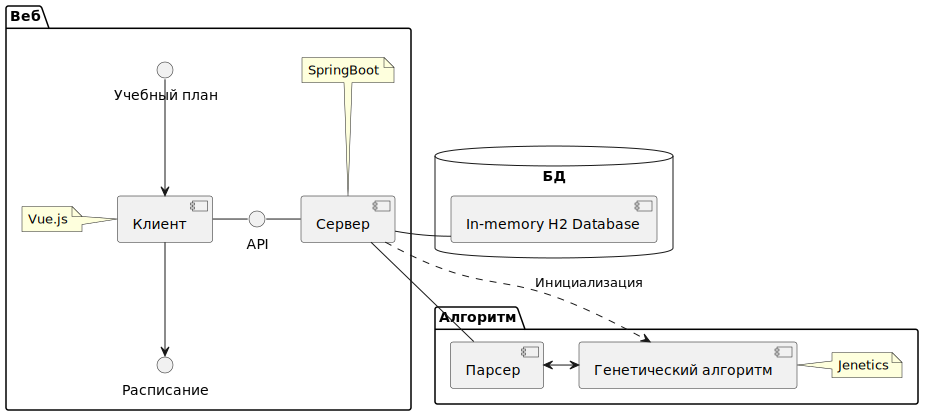
\includegraphics[height=0.40\linewidth]{images/seqDiag.svg}
\end{figure}
\end{frame}

\begin{frame}
\frametitle{Входные данные}
Учебный план в формате JSON
\begin{figure}
    \centering
    
\includegraphics[height=0.25\linewidth]{images/input_format.png}
\end{figure}
\end{frame}

\section{Анализ результатов}

\begin{frame}
\frametitle{Пример расписания}
\begin{figure}
\centering
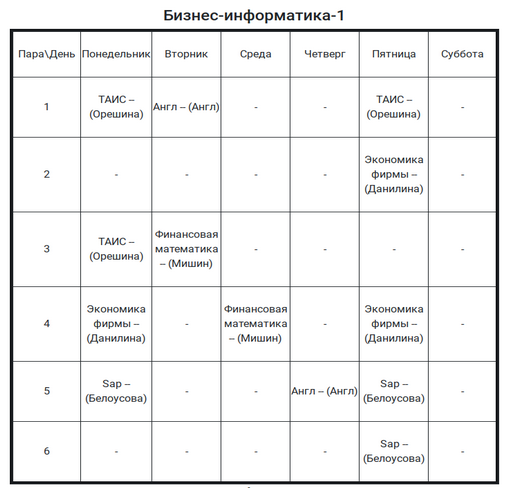
\includegraphics[scale=0.35]{images/timetable.png}    
\end{figure}
\end{frame}

\begin{frame}[c]
\frametitle{Сравнение методов селекции}
\begin{table}
\centering
\begin{tabular}{||c|c|c|c||}
\hline
                    & Рулеточная    &   Турнирная   &   Отсечения \\
\hline
Время селекции, с.      & 0.188         &   0.151       &   0.21      \\
\hline
Ср. целевой ф-ции   & 8.39          &   8.71        &   10.09     \\
\hline
Ср. возраст особи   & 1.11          &   1.43        &   14.21     \\
\hline
Формула             & $p_i = \frac{f_i}{\sum^N_{i=1}f_i}$ 
                                    & $\underset{\text{group of t from N}}{max} f_i $
                                                    & $\underset{\text{t of N}}{best}f_i$ \\
\hline
\end{tabular}
\end{table}
\end{frame}
\begin{frame}
\frametitle{Литература и источники}
\begin{enumerate}
\item Лазарев, А.А, Гафаров, Е. Р. Теория расписаний, задачи и алгоритмы // Учебник. – 2011. – С. 52–81.
\item Wilhelmstötter, F. // Jenetics Library User’s Manual 7.1 – 2022 – С.6–31, 54–67.
\item Lalescu L. // The description of the FET timetable generation algorithm [Электронный ресурс] – URL: https://lalescu.ro/liviu/fet/doc/en/generation-algorithm-description.html. (Дата обращения: 27.06.2022)
\item Разработка автоматизированной системы составления и оптимизации расписания занятий / Т.В. Сиркин, А.П. Чернышова, П.А. Мартынов, А.Д. Морозов // Молодой ученый. –2020. – С. 65-71.

\end{enumerate}
\end{frame}


\begin{frame}
\frametitle{Публикации и выступления}
\begin{itemize}
	\item Конгресс Молодых учёных 
        \begin{itemize}
            \item Победа в номинации "За лучший доклад молодого учёного" в секции "Информационные технологии"
            \item Публикация в сборнике тезисов
            \item Рекомендован к публикации статьи в Сборнике трудов Конгресса (входит в РИНЦ)
        \end{itemize}
	\item Конференция "Цифровая трансформация управления: проблемы и решения" 
    \item Студенческая олимпиада "Газпром"
        \begin{itemize} \item Победитель в конкурсе проектов в секции "Информационные системы и технологии"\end{itemize}
\end{itemize}
\end{frame}
\end{document}
